\documentclass[ngerman,hyperref={pdfpagelabels=false}]{beamer}

% -----------------------------------------------------------------------------

\graphicspath{{images/}}

% -----------------------------------------------------------------------------

\usetheme{KIT}

\setbeamercovered{transparent}
%\setbeamertemplate{enumerate items}[ball]

\newenvironment<>{KITtestblock}[2][]
{\begin{KITcolblock}<#1>{#2}{KITblack15}{KITblack50}}
{\end{KITcolblock}}

\usepackage[ngerman,english]{babel}
\usepackage[utf8]{inputenc}
\usepackage[TS1,T1]{fontenc}
\usepackage{array}
\usepackage{multicol}
\usepackage[absolute,overlay]{textpos}
\usepackage{beamerKITdefs}

\pdfpageattr {/Group << /S /Transparency /I true /CS /DeviceRGB>>}	%required to prevent color shifting withd transparent images


\title{Algorithmen I - Tutorium 4}
\subtitle{Sebastian Schmidt -- \textit{isibboi@gmail.com}}

\author[Sebastian Schmidt]{Sebastian Schmidt}
\institute{Arbeitsgruppe Kryptographie und Sicherheit}

\TitleImage[width=\titleimagewd,height=\titleimageht]{titel}

\KITinstitute{Arbeitsgruppe Kryptographie und Sicherheit}
\KITfaculty{Fakult\"at f\"ur Informatik}

% -----------------------------------------------------------------------------

\begin{document}
\setlength\textheight{7cm} %required for correct vertical alignment, if [t] is not used as documentclass parameter


% title frame
\begin{frame}
  \maketitle
\end{frame}

\begin{frame}{Wahrscheinlichkeitstheorie}
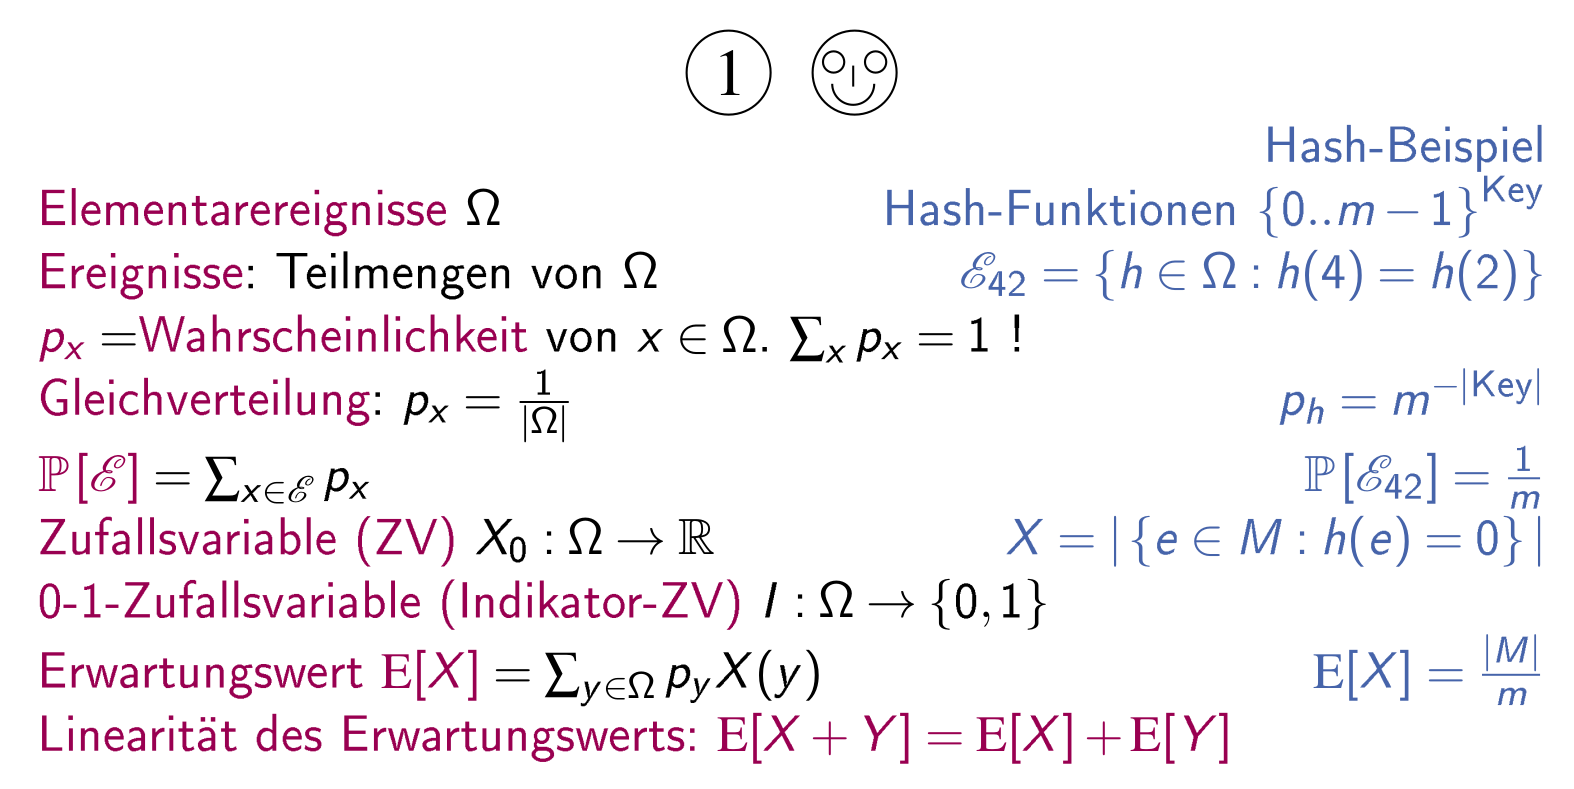
\includegraphics[width=\textwidth]{WT}
\end{frame}

\begin{frame}{Hashing mit einfach verketteten Listen}
\begin{itemize}[<+->]
\item Hashtabelle mit $h_n(x) := x \mod n$
\begin{itemize}
\item Wie groß sollte die Hashtabelle sein?
\item Gegeben $\{36, 78, 50, 1, 92, 15, 43, 99, 64\}$. Füge diese Zahlen in eine Hashtabelle mit Hashfunktion $h_5$ und $h_7$ ein.
\end{itemize}
\item Gebt Beispiele für gute und schlechte Hashfunktionen
\item Laufzeiten: \texttt{insert}, \texttt{find} und \texttt{remove}
\end{itemize}
\end{frame}

\begin{frame}{Anwendungsbeispiele für Hashtabellen}
Hashtabellen sind besser als Bäume, wenn man die erwartete Laufzeit betrachtet.
\begin{itemize}
\item<2-> Fallen euch konkrete Beispiele oder Gegenbeispiele ein?
\end{itemize}
\end{frame}

\begin{frame}{Beweis über Worst-Case}
Seien $m, n \in \mathbb{N}$.
$n$ ist die Anzahl der Elemente, die in eine Hashtabelle der Größe $m$ eingefügt werden.

Sei $U$ ein Universum mit $|U| \geq mn$.

Zeige, dass eine Teilmenge $M \subset U$ existiert mit $|M| \geq n$, sodass alle Elemente aus $M$ dem selben Slot der Hashtabelle zugeordnet werden.
\end{frame}

\begin{frame}{Verbesserung des Worst-Case}
\textit{\glqq Nach dem dritten Glas Bier behauptet ein Kommilitone, man könne Hashing mit verketteten Listen entscheidend verbessern, indem man die verketteten Listen stets sortiert halte.\grqq}

\begin{itemize}[<+->]
\item Wie ändert sich dadurch die Worst-Case Laufzeit von \texttt{insert}, \texttt{find} und \texttt{remove}?
\end{itemize}
\end{frame}


\end{document}
